\documentclass{standalone}
% tkz-tab: variation table (sign line + variation line). The derivative row
% label is text-mode on purpose: a math prime is a superscript glyph, which
% would pull the script-size symbol font (cmsy7) that the closure does not
% ship (fmt-preload rule); everything here stays at normalsize math.
\usepackage{tkz-tab}
\begin{document}
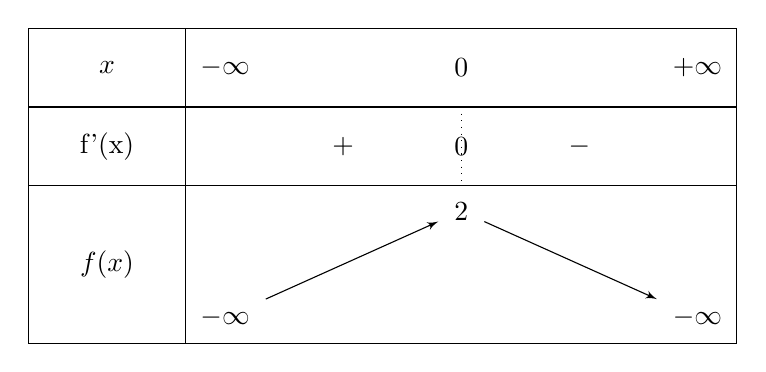
\begin{tikzpicture}
\tkzTabInit{$x$/1, f'(x)/1, $f(x)$/2}{$-\infty$, $0$, $+\infty$}
\tkzTabLine{, +, z, -, }
\tkzTabVar{-/{$-\infty$}, +/{$2$}, -/{$-\infty$}}
\end{tikzpicture}
\end{document}
